\documentclass[10pt]{beamer}

\usetheme[progressbar=frametitle]{metropolis}

\usepackage[compatibility=false]{caption}
\usepackage{subcaption}

\usepackage{booktabs}
\usepackage{hyperref}
\usepackage[scale=2]{ccicons}
\usepackage{tikz}
\usetikzlibrary{positioning}
\usetikzlibrary{3d}

\usepackage{pgfplots}
\usepgfplotslibrary{dateplot}

\usepackage{xspace}
\newcommand{\themename}{\textbf{\textsc{metropolis}}\xspace}

\title{Evolvability in EANN}
\subtitle{Northwest Honors Research Symposium}
\date{November 5th, 2016}
\author{\texorpdfstring{Matthew Moreno$^{*}$\newline\url{mamoreno@pugetsound.edu}}{Matthew Moreno}}
\institute{$^{*}$University of Puget Sound}
\titlegraphic{\hfill\includegraphics[height=2cm]{img/UofPS_stacked_maroonRGB_PNG.png}}

\begin{document}

\maketitle

% \begin{frame}{Table of contents}
%   \setbeamertemplate{section in toc}[sections numbered]
%   \tableofcontents[hideallsubsections]
% \end{frame}

\section{Motivation}

\begin{frame}{Bio AI}
\begin{itemize}
  \item tasks that are easy for people can be very difficult for computers
  \item idea: use algorithms inspired by biological structures and processes
%   \item significant growth in recent years (especially with cheap parallel computing power)
\end{itemize}
\end{frame}

\begin{frame}{Bio AI}
\begin{figure}
\includegraphics[width=\textwidth]{img/AlexClassification.png}
\captionsetup{singlelinecheck=off,justification=raggedright}
\caption{TensorFlow Image Identification \cite{ImageRecognition}}
\end{figure}
\end{frame}

\begin{frame}{Bio AI}
\begin{figure}
\includegraphics[width=0.8\textwidth]{img/unexpected-images-tested-with-imageidentify.png}
\captionsetup{singlelinecheck=off,justification=raggedright}
\caption{Amusing responses to unexpected images from the Wolfram Image Identification Project \cite{Wolfram2015WolframProject}}
\end{figure}
\end{frame}

\begin{frame}{Bio AI}
\begin{figure}
  \includegraphics[width=0.6\textwidth]{img/before_after_deepdream}
\captionsetup{singlelinecheck=off,justification=raggedright}
\caption{Google Deep Dream \cite{Mordvintsev2015DeepDreamNetworks}}
\end{figure}
\end{frame}


\begin{frame}{Bio AI}
\begin{figure}
  \includegraphics[width=0.8\textwidth]{img/neural_network_schematic}
  \captionsetup{singlelinecheck=off,justification=raggedright}
  \caption{Schematic diagram of an Artificial Neural Network (ANN) \cite[Figure 1]{Ata2015ArtificialReview}}
\end{figure}
\end{frame}

% \begin{frame}{Bio AI}
% shortcomings of backpropagation
% \begin{itemize}
%   \item supervised learning
%   \item no online modification
% \end{itemize}
% \end{frame}



\section{Evolutionary Algorithms}

\begin{frame}{Evolutionary Algorithms}
\begin{figure}
  \includegraphics[width=0.8\textwidth]{img/working_principle_of_EA.png}
  \captionsetup{singlelinecheck=off,justification=raggedright}
  \caption{Schematic illustration of the evolutionary algorithm \cite[Figure 1]{Prothmann2009EvolutionaryOptimisation}}
\end{figure}
    
\end{frame}

\begin{frame}{Evolutionary Algorithms}
\begin{figure}
  \includegraphics[width=0.8\textwidth]{img/evolution_in_action.png}
  \captionsetup{singlelinecheck=off,justification=raggedright}
\href{https://youtu.be/z9ptOeByLA4?t=1m08s}{\caption{Evolution in Action \cite{Cheney2013UnshacklingEncoding}}}
\end{figure}
\end{frame}

\begin{frame}{Evolutionary Algorithms: Glossary}
\begin{itemize}
  \item individual
  \item population
  \item fitness function
  \item selection
  \item recombination
  \item genotype
  \item phenotype
\end{itemize}
\end{frame}

\begin{frame}{Evolutionary Algorithms: Problem Statement}
  What makes an evolutionary algorithm work?
\end{frame}

\section{Defining Evolvability}

\begin{frame}{Defining Evolvability}
consensus: the amount of useful variation generated by the evolutionary process
\begin{itemize}
  \item evolvability as the ability to generate heritable variation
  \item evolvability as bias towards useful variation
\end{itemize}
\end{frame}

% \begin{frame}{The Evolvability Conundrum}
% How can natural selection ``favor properties hat may prove useful to a given lineage in the future, but have no present adaptive function''? \cite{Pigliucci2008IsEvolvable}
% \end{frame}


\subsection{Evolvability as Heritable Variation}

\begin{frame}{Evolvability as Heritable Variation}
	\begin{figure}
 \centering
    \begin{subfigure}[b]{0.5\textwidth}
        \centering
    	\includegraphics[width=\textwidth]{img/individual_evolvability.png}
        \caption{high individual evolvability}
        \label{subfig:canalization}
    \end{subfigure}%
    \hfill
    \begin{subfigure}[b]{0.5\textwidth}
        \centering
        \includegraphics[width=\textwidth]{img/low_individual_evolvability.png}
        \caption{low individual evolvability}
        \label{subfig:no_canalization}
    \end{subfigure}
 	\captionsetup{singlelinecheck=off,justification=raggedright}
    \vspace{-4ex}
  \captionsetup{singlelinecheck=off,justification=raggedright}
  \caption{An illustration of individual evolvability, considering evolvability as heritable variation \cite{Wilder2015ReconcilingEvolvability}.}
  \label{fig:high_vs_low_individual_evolvability}
\end{figure}
\end{frame}

\begin{frame}{Evolvability as Heritable Variation}
  \begin{figure}
 \centering
    \begin{subfigure}[b]{0.5\textwidth}
        \centering
    	\includegraphics[width=\textwidth]{img/individual_evolvability}
        \caption{individual evolvability}
        \label{subfig:individual_evolvability}
    \end{subfigure}%
    \hfill
    \begin{subfigure}[b]{0.5\textwidth}
        \centering
        \includegraphics[width=\textwidth]{img/population_evolvability}
        \caption{population evolvability}
        \label{subfig:population_evolvability}
    \end{subfigure}
 	\captionsetup{singlelinecheck=off,justification=raggedright}
    \vspace{-4ex}
  \captionsetup{singlelinecheck=off,justification=raggedright}
  \caption{An illustration contrasting individual and population evolvability \cite{Wilder2015ReconcilingEvolvability}.}
  \label{fig:individual_vs_population_evolvability}
\end{figure}
\end{frame}

\subsection{Evolvability as Bias towards Useful Variation}

\begin{frame}{Evolvability as Bias towards Useful Variation}
  \begin{figure}
    \centering
    \includegraphics[width=0.8\textwidth]{img/developmental_constraint}
 	\captionsetup{singlelinecheck=off,justification=raggedright}
  	\caption{Illustration of developmental constraint; high evolvability left and low evolvability right \cite{Smith1985DevelopmentalBiology,Tuinstra1990LackDevelopment}.}
    \label{fig:developmental_constraint}
\end{figure}
\end{frame}

\begin{frame}{Evolvability as Bias towards Useful Variation}
  \begin{figure}
    \centering
    \includegraphics[width=0.8\textwidth]{img/exploratory_growth}
 	\captionsetup{singlelinecheck=off,justification=raggedright}
  	\caption{Illustration of exploratory growth; high evolvability left and low evolvability right \cite{Downing2015IntelligenceSystems}.}
    \label{fig:exploratory_growth}
\end{figure}
\end{frame}

\begin{frame}{Evolvability as Bias towards Useful Variation}
  \begin{figure}
    \centering
    \includegraphics[width=0.8\textwidth]{img/robustness}
 	\captionsetup{singlelinecheck=off,justification=raggedright}
  	\caption{Illustration of robustness; high evolvability left and low evolvability right \cite{Downing2015IntelligenceSystems}.}
    \label{fig:robustness}
\end{figure}
\end{frame}


\section{Promoting Evolvability}

\subsection{Indirect Representation}

\begin{frame}{Promoting Evolvability: Indirect Representation}
  \begin{figure}
  \centering
  \begin{subfigure}[b]{0.5\textwidth}
    \centering
    \includegraphics[width=\textwidth]{img/direct_encoding.png}
    \caption{direct encoding (low regularity)}
    \label{subfig:canalization}
  \end{subfigure}%
  \hfill
  \begin{subfigure}[b]{0.5\textwidth}
    \centering
    \includegraphics[width=\textwidth]{img/cppn-neat_encoded.png}
    \caption{indirect encoding (high regularity)}
  \end{subfigure}
  \captionsetup{singlelinecheck=off,justification=raggedright}
  \caption{Representative examples of soft robots evolved with direct and indirect representations \cite[Figures 6, 7]{Cheney2013UnshacklingEncoding}}
  \label{fig:direct_irregular_vs_indirect_regular}
\end{figure}
\end{frame}


% \begin{frame}{Indirect Encodings}
% \begin{figure}
%   \includegraphics[width=0.6\textwidth]{img/neurogram.png}
%   \captionsetup{singlelinecheck=off,justification=raggedright}
%   \caption{\cite{Ha2015Neurogram}}
% \end{figure}
% \end{frame}

\subsection{Selection Pressure}

% \begin{frame}{Selection Pressure}
% \begin{itemize}
%   \item modularly differing fitness function \cite{Reisinger2005TowardsEvolvability}
%   \item average performance of local genetic environment \cite{Reisinger2005TowardsEvolvability}
%   \item direct selection (i.e. evolvability selection, novelty search)
% \end{itemize}
% \end{frame}

\begin{frame}{Promoting Evolvability: Selection Pressure}
  \begin{figure}
  \includegraphics[width=\textwidth]{img/varying_fitness_function}
  \captionsetup{singlelinecheck=off,justification=raggedright}
  \caption{An illustration of a modularly varying fitness function \cite{Kashtan2005SpontaneousMotifs}}
  \label{fig:hummingbird_selection_pressure}
\end{figure}
\end{frame}



\section{Promoting Evolvability in EANN} \label{sec:eann}

\begin{frame}{HyperNEAT}
\begin{figure}
	 \begin{tikzpicture}
    \node (first) {\includegraphics[width=0.25\textwidth]{img/cppn}};
    \node (second) [right=of first] {\includegraphics[width=0.25\textwidth]{img/walking_fish}};
    \node (third) [right=of second] {\includegraphics[width=0.25\textwidth]{img/neural_network}};

    \node (a) [right=of first] {};
    \node (b) [left=of second] {};
    \node (c) [right=of second] {};
    \node (d) [left=of third] {};

    \draw [ultra thick,->] (b) to (a);
    \draw [ultra thick,->] (d) to (c);
\end{tikzpicture}
    \captionsetup{singlelinecheck=off,justification=raggedright}
    \vspace{-4ex}
  	\caption{The working principle of HyperNEAT indirect genetic encoding; the genotype, a Compositional Pattern Producing Network (left), is used to construct a neural network configuration (right) \cite{Ha2015Neurogram}, \cite[Figure 15]{Clune2011OnRegularity}}
\end{figure}
\end{frame}

\begin{frame}{Novelty Search}
   \begin{figure}
  \includegraphics[width=0.8\textwidth]{img/novelty_search}
  \captionsetup{singlelinecheck=off,justification=raggedright}
  \caption{Novelty search, an example of divergent selection \cite{Wilder2015ReconcilingEvolvability}}
\end{figure}
\end{frame}

\section{Conclusion}

\begin{frame}{Closing Thoughts}
Potential Applications
\begin{itemize}
  \item robotic control \cite{Fehervari2010EvolvingRobots}
  \item financial trading \cite{Sher2011EvolvingAgents}
  \item long term: more general artificial intelligence? \cite[pg 364]{Downing2015IntelligenceSystems}
\end{itemize}
Scientific Questions
\begin{itemize}
  \item what are the fundamental mechanisms at play in cognition and evolution?
\end{itemize}
\end{frame}

\appendix

\begin{frame}{Acknowledgements}
\begin{itemize}
\item My thesis advisor, Professor Chambers
\item Professor Smith for serving as a reader for my thesis
\item Professor Erving for his support as the Honors Program Director
\item Seattle Pacific University for hosting the Northwest Honors Research Symposium
\end{itemize}
\begin{columns}[T,onlytextwidth]
\column{\textwidth}
\begin{minipage}[]{0.15\textwidth}
~
\end{minipage}%
\begin{minipage}[]{0.3\textwidth}
    \begin{centering}
    \includegraphics[width = \textwidth]{img/SPUTorch_208_LR}
    \end{centering}
\end{minipage}%
\begin{minipage}[]{0.1\textwidth}
~
\end{minipage}%
\begin{minipage}[]{0.3\textwidth}
	\begin{centering}
    \includegraphics[width = \textwidth]{img/UofPS_stacked_maroonRGB_PNG}
    \end{centering}
\end{minipage}%
\begin{minipage}[]{0.15\textwidth}
~
\end{minipage}%
\end{columns}
\end{frame}

\begin{frame}[standout]
  Questions?
\end{frame}

\begin{frame}[allowframebreaks]{References}

  \bibliography{Mendeley}
  \setbeamertemplate{bibliography item}{\insertbiblabel}
  %\nocite{*} % Insert publications even if they are not cited in the poster
  \bibliographystyle{apalike}
\end{frame}

\begin{frame}{Bio AI}
\begin{figure}
  \includegraphics[width=0.6\textwidth]{img/nn_art_styles.png}
  \captionsetup{singlelinecheck=off,justification=raggedright}
  \caption{A Neural Algorithm of Artistic Style \cite{Gatys2015AStyle}}
\end{figure}
\end{frame}

\begin{frame}{Evolvability as Heritable Variation}
  \begin{figure}
 \centering
    \begin{subfigure}[b]{0.5\textwidth}
        \centering
    	\includegraphics[width=\textwidth]{img/individual_evolvability}
        \caption{individual evolvability}
        \label{subfig:individual_evolvability}
    \end{subfigure}%
    \hfill
    \begin{subfigure}[b]{0.5\textwidth}
        \centering
        \includegraphics[width=\textwidth]{img/population_evolvability}
        \caption{population evolvability}
        \label{subfig:population_evolvability}
    \end{subfigure}
 	\captionsetup{singlelinecheck=off,justification=raggedright}
    \vspace{-4ex}
  \captionsetup{singlelinecheck=off,justification=raggedright}
  \caption{An illustration contrasting individual and population evolvability \cite{Wilder2015ReconcilingEvolvability}.}
  \label{fig:individual_vs_population_evolvability}
\end{figure}
\end{frame}

\begin{frame}{Evolvability as Bias towards Useful Variation}
  \begin{figure}
    \centering
    \includegraphics[width=0.8\textwidth]{img/exploratory_growth}
 	\captionsetup{singlelinecheck=off,justification=raggedright}
  	\caption{Illustration of exploratory growth; high evolvability left and low evolvability right \cite{Downing2015IntelligenceSystems}.}
    \label{fig:exploratory_growth}
\end{figure}
\end{frame}

\begin{frame}{Evolvability as Bias towards Useful Variation}
  \begin{figure}
    \centering
    \includegraphics[width=0.8\textwidth]{img/robustness}
 	\captionsetup{singlelinecheck=off,justification=raggedright}
  	\caption{Illustration of robustness; high evolvability left and low evolvability right \cite{Downing2015IntelligenceSystems}.}
    \label{fig:robustness}
\end{figure}
\end{frame}

\begin{frame}{Selection Pressure}
\begin{figure}
\resizebox{\textwidth}{!}{%
	\pgfmathsetseed{1}
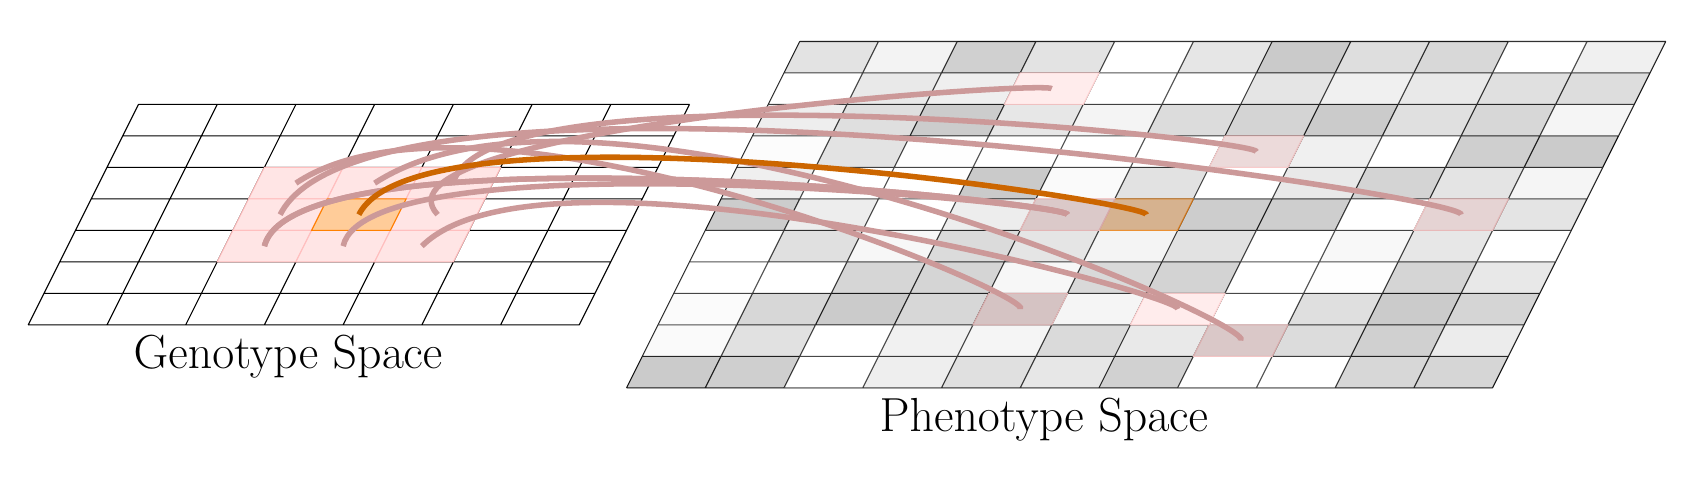
\begin{tikzpicture} [x={(-0.2cm,-0.4cm)}, y={(1cm,0cm)}, z={(0cm,1cm)}, scale=1]   

   \begin{scope}[canvas is yx plane at z=0]
     \draw [black!100] (0,2) grid (7,9);
     \draw [black!100] (8,0) grid (19,11);
     
     % primary phenotype mapping
     \foreach \x in {2,3,4}
       \foreach \y in {4,5,6}
    	  \filldraw[fill=pink!40!white, draw=pink] (\x, \y) rectangle (\x+1,\y+1);

     \filldraw[fill=orange!40!white, draw=orange] (3, 5) rectangle (4,6);
     \filldraw[fill=orange!40!white, draw=orange] (13, 5) rectangle (14,6);

      
     \foreach \cx/\cy/\dx/\dy in {2.5/4.5/12.5/8.5,3.5/4.5/15.5/9.5,4.5/4.5/14.5/3.5,2.5/5.5/17.5/5.5,4.5/5.5/11.5/1.5,2.5/6.5/12.5/5.5,2.5/6.5/12.5/5.5,3.5/6.5/12.5/5.5,4.5/6.5/14.5/8.5}
      	\filldraw[fill=pink!40!white, draw=pink] (\dx-0.5, \dy-0.5) rectangle (\dx+0.5,\dy+0.5);
        
      \foreach \x in {8,9,...,18}
       \foreach \y in {0,1,...,10}
        \pgfmathparse{0.9*rnd+0.3}
        \definecolor{MyColor}{rgb}{\pgfmathresult,\pgfmathresult,\pgfmathresult}
        \fill[fill=MyColor, opacity = 0.3] (\x,\y) rectangle (\x+1,\y+1);

      \foreach \cx/\cy/\dx/\dy in {2.5/4.5/12.5/8.5,3.5/4.5/15.5/9.5,4.5/4.5/14.5/3.5,2.5/5.5/17.5/5.5,4.5/5.5/11.5/1.5,2.5/6.5/12.5/5.5,2.5/6.5/12.5/5.5,3.5/6.5/12.5/5.5,4.5/6.5/14.5/8.5}
     	\draw [pink!80!black, line width=2pt] (\cx, \cy) to[bend right=90, in looseness=0.1] (\dx, \dy);

       \draw [orange!80!black, line width=2pt] (3.5,5.5) to[bend right=90, in looseness=0.1] (13.5,5.5);
     
     \draw [black] (3.5,10)node {\LARGE Genotype Space};
     \draw [black] (13.5,12)node {\LARGE Phenotype Space};

   \end{scope}
 \end{tikzpicture}
}
\captionsetup{singlelinecheck=off,justification=raggedright}
\caption{average performance of local genetic environment \cite{Reisinger2005TowardsEvolvability}}
\end{figure}
\end{frame}

\begin{frame}{Bio AI}
\begin{figure}
  \includegraphics[width=\textwidth]{img/iterative_places}
\captionsetup{singlelinecheck=off,justification=raggedright}
\caption{Google Deep Dream \cite{Mordvintsev2015Inceptionism:Networks}}
\end{figure}
\end{frame}

% \begin{frame}{Measuring Evolvability}
% \begin{itemize}
%   \item amount of information able to acquire (different speeds of varying fitness function)\cite{Reisinger2005TowardsEvolvability} 
%   \item RMS distance in behavioral characterization space (population diversity), ``We approximate an individual’s capacity to generate
% future phenotypic variation by measuring phenotypic
% variability among a sample of the individual’s simulated off-
% spring (which are discarded). Such variability is quantified as
% the number of unique behaviors; in particular, each offspring
% is considered sequentially and added to a list of unique behaviors
% only if its behavior is significantly different from the
% behaviors of organisms already in the list. Two behaviors are
% considered different if the distance between them according
% to a domain-specific behavioral distance metric is above a
% pre-specified threshold'' \cite{Mengistu2016EvolvabilityIt}
%   \item ``a measurement of evolvability should characterize the
% amount of variability that can be accessed in an individual or population's genetic neighborhood; number of distinct phenotypes in a genetic neighborhood around individual; amounts to Monte Carlo sampling of the phenotypic space surrounding an individual \cite{Wilder2015ReconcilingEvolvability}
%   %\item \cite{Tarapore2015EvolvabilityBenchmarks}
% \end{itemize}
% \end{frame}

\section{Experiment}

\begin{frame}{Development and the Environment}
  \begin{figure} \label{fig:elephant_developmental_perturbation}
  \includegraphics[width=0.8\textwidth]{img/elephant_developmental_perturbation.jpg}
  \captionsetup{singlelinecheck=off,justification=raggedright}

  \caption{An illustration of canalization against environmental perturbation}
\end{figure}
\end{frame}

\begin{frame}{Development and the Environment}
  \begin{figure} \label{figs/plant_developmental_perturbation}
  \includegraphics[width=0.8\textwidth]{img/plant_developmental_perturbation.jpg}
  \captionsetup{singlelinecheck=off,justification=raggedright}
  \caption{An illustration alternate phenotypes expressed based on environmental signals}
\end{figure}

\end{frame}


\end{document}
